\chapter{Représentations numériques}

\minitoc

\section{Notion de bases ou radix}

\subsection{Décomposition en puissance de la base}
Les nombres que nous manipulons tous les jours s'expriment en base (ou {\it radix}) $10$.
On parle de base $10$ car on utilise $10$ symboles (appelés {\it chiffres}) allant de $0$ à $9$ inclus.
Par la suite, on s'autorisera à parler de $digits$.
Dans un nombre, ces digits sont en fait des {\it coefficients} du système décimal :
pour former un nombre, on multiplie ces coefficients par les puissances successives de $10$.
Par exemple le nombre $142$ s'exprime ainsi :

$$ 142 = 1\times 10^2 + 4\times 10^1 + 2\times 10^0$$

Il en est de même des nombres fractionnaires comme :
$$ 142.34 = 1\times 10^2 + 4\times 10^1 + 2\times 10^0 + 3\times 10^{-1} + 4\times 10^{-2}$$

La formule générale pour la base $10$ est bien entendu :
$$ x = \sum_{i=-\infty}^{i=\infty} c_i.10^i, \mbox{avec } c_i \in \{0\dots 9\}$$
et se généralise pour toute base $r$ :
$$ x = \sum_{i=-\infty}^{i=\infty} c_i.r^i, \mbox{avec } c_i \in \{0\dots (r-1)\} $$

Les ordinateurs n'utilisent pas la base $10$, mais la base $2$, qui ne possède que deux valeurs de
coefficients possibles : $0$ et $1$. De plus, ces ordinateurs ne peuvent stocker un nombre infini de digits et devront passer par
une représentation des nombres avec un nombre fini de digits

Afin d'éviter toute confusion par la suite, nous plaçons en indice du nombre l'indication de la base utilisée,
ce qui évitera de nous perdre lors des changements de base. Par exemple, on peut noter :
$$10110_{10} = 10011101111110_2$$

En pratique, il existe deux autres bases indispensables aux informaticiens et électroniciens : la base octale (base 8) et la base
hexadécimale (base 16). La première n'utilise que les digits allant de $0$ à $7$. En hexadécimal, on doit introduire
de nouveaux symboles au delà du $9$ : on utilise --dans l'ordre-- les lettres (majuscules ou minuscules) A, B, C, D,
E et F, correspondant respectivement à 10,11,12,13,14 et 15. La table suivante montre les 18 premiers nombres dans
le système décimal, binaire, octal et hexadécimal, ainsi que deux autres représentations sur lesquelles nous
reviendrons un peu plus tard).\\

\begin{table}
 \centering
  \begin{tabular}{ | r | r | r | r | r | r |}
    \hline
    \multicolumn{6}{|c|}{base (ou nom du code)} \\
    \hline
    10 & 2 & 8 & 16 & BCD & Gray \\ \hline \hline
   0 &     0 &     0 &     0 &  0000 &     0 \\ \hline
   1 &     1 &     1 &     1 &  0001 &     1 \\ \hline
   2 &    10 &     2 &     2 &  0010 &    11 \\ \hline
   3 &    11 &     3 &     3 &  0011 &    10 \\ \hline
   4 &   100 &     4 &     4 &  0100 &   110 \\ \hline
   5 &   101 &     5 &     5 &  0101 &   111 \\ \hline
   6 &   110 &     6 &     6 &  0110 &   101 \\ \hline
   7 &   111 &     7 &     7 &  0111 &   100 \\ \hline
   8 &  1000 &    10 &     8 &  1000 &  1100 \\ \hline
   9 &  1001 &    11 &     9 &  1001 &  1101 \\ \hline
  10 &  1010 &    12 &     a & 00010000 &  1111 \\ \hline
  11 &  1011 &    13 &     b & 00010001 &  1110 \\ \hline
  12 &  1100 &    14 &     c & 00010010 &  1010 \\ \hline
  13 &  1101 &    15 &     d & 00010011 &  1011 \\ \hline
  14 &  1110 &    16 &     e & 00010100 &  1001 \\ \hline
  15 &  1111 &    17 &     f & 00010101 &  1000 \\ \hline
  16 & 10000 &    20 &    10 & 00010110 & 11000 \\ \hline
  17 & 10001 &    21 &    11 & 00010111 & 11001 \\ \hline
  \end{tabular}
  \caption{Table des correspondances entre bases $10$, $2$, $8$, $16$, puis code BCD et code de Gray}
\end{table}

Enfin, notons qu'il existe des bases plus exotiques. Par exemple, la numération mésopotamienne (utlisée par babyloniens notamment),
a recours à la base 60 : c'est la base sexagésimale. Elle date d'environ 3000 ans avant notre ère ! On en retrouve quelques vestiges dans notre système horaire et dans la mesure des angles.
A titre de curiosité, la figure \ref{sexa} présente une pierre datant du \siecle{17} siècle avant Jésus-Christ.
Elle démontre la maîtrise du calcul de $\sqrt 2$, dans cette base sexagésimale : les archéologues nous enseignent que cette tablette
vise à établir l'égalité suivante, calculée il y a près de 38 siècles !
$$\sqrt 2 \approx 1.414212=1+\frac{24}{60}+\frac{51}{60^2}+\frac{10}{60^3}=\frac{30547}{21600}$$
\begin{figure}[htb]
  \begin{center}
    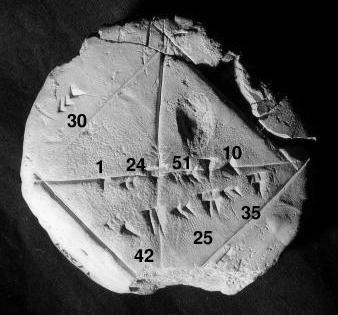
\includegraphics[width=4cm]{./figures/Ybc7289-bw.jpg}
    \caption{(Wikipedia) Tablette avec l'écriture en numération sexagésimale de 1/2 et des valeurs approchées au six dix-millionièmes de $\sqrt 2$, ainsi que :
    $\frac{\sqrt 2}{2}=42+\frac{20}{60}+\frac{35}{60^2}+\frac{35}{60^2}=\frac{30547}{720}$}
    \label{sexa}
  \end{center}
\end{figure}

\paragraph{Nombre de bits nécessaires pour représenter un entier $x$}
On déduit aisément le nombre de bits $n$ nécessaires à la représentation d'un entier $x$ :
pour $n$ bits, on a $x \leq 2^n-1 < 2^n$, d'où $log_2(x)<n$.
Avec $n\in \mathbb(N)$, on déduit \fbox{$n=\floor*{log_2(x)}+1$}, où $\floor*{\alpha}$ représente le plus petit entier inférieur à $\alpha$.

\paragraph{Erreur de calcul liés aux représentations}
Nous verrons très bientôt que les ordinateurs sont capables d'effectuer les calculs traditionnels de l'arithmétique, au sein d'une Unité Arithmétique et Logique (UAL).
Le nombre de bits des opérandes en entrée de cette UAL sont limités (8,16, 32 voire 64 bits). Les calculs réalisés {\it directement} (matériellement) par les ordinateurs seront
forcément entachés d'erreurs liées à ces limitations, dont l'ingénieur devra se méfier. Notons toutefois que tous les langages possèdent des bibliothèques qui permettent
d'augmenter le nombre de digits manipulés de manière logicielle, avec un surcoût important en terme de temps de calcul :
il s'agit de l'arithmétique "multi-précision" plus communément appelée {\it arbitrary-precision arithmetic} ou {\it bignum}.
Les temps de
calculs en bignum conduit la plupart des scientifiques à ne pas les utiliser et à se limiter au calcul fourni directement par la machine..

\subsection{Conversion entre bases}
Grâce aux formules précédentes, nous savons transformer un nombre exprimé dans une base {\it r} en en nombre décimal.
Il est à présent important de savoir faire l'inverse, à savoir : convertir un nombre décimal $x_{10}$ vers tout autre base {\it r} .
Ceci peut se faire de manière mécanique : il suffit de diviser le nombre $x$ (dividende) par $r$ (diviseur), puis de répéter
l'opération sur le quotient jusqu'à ce que ce quotient soit nul. Le premier reste obtenu sera le digit
le plus à droite (En base  binaire, on parle de LSB : least significant bit), et le dernier reste  le digit le plus à gauche
(MSB : most significant bit).

Dans le cas de nombres fractionnaires, il faut procéder de la manière suivante : multiplier le nombre par $r$ jusqu'à obtenir
un nombre sans partie fractionnaire. Ceci n'est évidemment pas toujours possible : selon les nombres en présence, ce calcul ne conduit pas
forcément à un nombre sans partie fractionnaire ! Notamment, il arrive fréquemment que des nombres, exprimables avec un nombre fini de digits dans une base,
puissent nécessiter un nombre {\it infini} de digits dans une autre base.

\subsection{Exemples}
\begin{itemize}
\item {\bf Convertir le nombre $12_{10}$ en binaire}\\
\underline{Solution:}\\
\begin{align*}
 12 / 2 &= 6 + 0 \\
  6 / 2 &= 3 + 0 \\
  3 /2  &= 1 + 1 \\
  1 / 2 &= 0 + 1
\end{align*}

Par conséquent :
$( 12 )_{10} = ( 1100 )_2$\\

\item {\bf Convertir $( 0.75)_{10}$ en binaire}\\
\underline{Solution:}\\
\begin{align*}
0.75 \times 2 &= 1.5 = 1 + 0.50 \\
0.50 \times 2 &= 1.0 = 1 + 0 \\
\end{align*}
Ainsi : $$( 0.75)_{10} = ( 0.11)_{2}$$\\

\item {\bf Convertir $( 0.39654 )_{10}$ en binaire}\\
\underline{Solution:}\\
\begin{align*}
0.39654 \times 2 &= 0.79308 = 0 + 0.79308 \\
0.79308 \times 2 &= 1.58616 = 1 + 0.58616 \\
0.58616 \times 2 &= 1.17232 = 1 + 0.17232 \\
0.17232 \times 2 &= 0.34464 = 0 + 0.34464 \\
\end{align*}
etc...Cette conversion n'a pas de fin. La partie fractionnaire ne peut s'exprimer sous la forme d'une somme exacte de puissance de $2$. On notera la solution :
$$( 0.39654 )_10 = ( 0.0110... )_2$$
\end{itemize}

Il est important que vous sachiez rapidement effectuer ces conversions avec votre ordinateur ou calculatrice préférée
\footnote{Pour votre information, il est possible d'utiliser Google pour effectuer cela : tapez ``0x123 in octal'' dans l'invite de Google...Vous obtenez $0o443$}.

\subsection{Conversions binaire, hexadécimal, octal}
Comme $2^4=16$, il s'en suit que la représentation binaire de chaque digit de la base $16$ nécessite $4$ bits. Pour la base octale, il en suffit de $3$.
De ce fait, les conversions de nombres binaires vers l'hexadécimal ou l'octal se réalisent simplement, par groupement de bits. En partant de la droite, il suffit par exemple de regrouper 4 bits pour obtenir un digit hexa. Par exemple :
$$\mbox{le nombre } 101101_2 = 10\_1101_2 = 0010\_1101_2=2D_{16}={\bf 0x2D}$$

Dans le cas de nombre fractionnaires, le sens de lecture s'inverse pour la partie fractionnaire. Ainsi :
$$\mbox{le nombre } 1011.01_2 = 1011.0100_2 = B.4_{16}$$

On procède de même pour la traduction octale.
$$( 10110001101011.1111 )_2 =(010\ 110\  001\  101\  011\  .\  111\  100)_2 = ( 26153.74 )_8$$

\subsection{Bits, bytes, nibbles, words}
La plus petite unité informatique est le bit, qui est l'abréviation de {\it binary digit}.
Toutefois rares sont les ordinateurs qui ne traitent qu'un seul bit à la fois : la plus petite la grandeur manipulable par la quasi-totalité des ordinateurs reste l'{\bf octet} : c'est l'aggrégation de 8 bits. Sa traduction anglaise est le {\it byte}, qui se prononce {\it bait} et qui ne doit pas être confondu avec le bit. Le regroupement de 4 bits est moins connu, mais indispensable : il s'agit du {\bf quartet} ou {\it nibble} en anglais. Nous verrons plus loin en quoi il est important. Enfin, on parle de {\bf mot} ou {\it word} pour le regroupement de 16 bits, sans toutefois que cette définition soit parfaitement admise. On parlera d'ailleurs de processeurs qui opèrent sur des mots de 16 bits, 32 bits, 64 bits etc...\\

Les bits des quartets, octets et mots sont généralement manipulés simultanément, lorsque la machine possède les circuits qui le permettent. Nous y reviendrons par la suite.

\paragraph{Première addition binaire}
Considérons le cas de l'addition binaire. Seuls 4 combinaisons sont à étudier :
\begin{align*}
0+0 &= 0 \\
0+1 &= 1 \\
1+0 &= 1 \\
1+1 &= 0 \mbox{ et une retenue de 1}
\end{align*}

Nous verrons, au chapitre suivant, comment forcer le silicium à réaliser électriquement ce calcul !






\section{Représentation des entiers négatifs.}

Jusqu'ici nous n'avons pas parlé de nombres négatifs. Comment représenter des nombres négatifs ? La manière la plus intuitive serait de considérer un nombre négatif comme la juxtaposition de deux informations représentées isolément :
le signe et la valeur absolue (``magnitude'').
Le signe pourrait n'être encodé que sur 1 seul bit : 0 ou 1 représentant par exemple le + et le - respectivement.
On appelle cette représentation "magnitude signée". Cette représentation "positionnelle" est tout à fait envisageable,
mais elle se révèle \textbf{inefficace matériellement}.
Elle oblige notamment à revoir le calcul de l'addition.
Elle a donc rapidement été abandonnée au cours de l'histoire de l'Informatique.
A l'inverse, certaines opérations sont grandement simplifiées par le recours à la \textbf{représentation complémentée} d'un nombre.
Aujourd'hui, les ordinateurs stockent les valeurs négative en binaire, en complément à 2.
Nous allons donc commencer par cette "bonne" représentation, puis nous reviendrons sur ces autres représentations obsolètes ou rares.

\subsection{Complément à $r$ d'un nombre}
Le complément à $r$ d'un entier $n$ sur $k$ digits, noté $C_{r,k}(n)$ est défini par :
$$"-n"_{r,k}=C_{r,k}(n)=r^k-n$$
Le nombre précédé de son signe négatif est écrit entre guillemet, car il ne s'agit que d'une convention "picturale" :
ce "-" n'est pas un digit de la base.\\

La formule fondamentale pour un nombre binaire se réduit donc à :

\begin{equation}
  \boxed{$$"-n"_{2,k}=C_{2,k}(n)=2^k-n$$}
\end{equation}

On a ainsi, pour un représentation de $-3$ en complément à 2, représenté sur 4 bits :
$$"-3"_{2,4}=C_{2,4}(3)=2^4-3=13=1101_2$$

On dit que 13 est le complément à 2 de 3 (et non $-3$) sur 4 bits.

\paragraph{Remarques}
\begin{enumerate}
  \item L'expression "complément à 2", fréquemment utilisée, est un raccourci langagier pour dire "complément à $2^k$" !
  \item Lorsqu'on augmente le nombre $k$ de digits autorisés dans la représentation, sa représentation change beaucoup, mais de manière structurée. Le signe se
  propage vers la gauche. En utilisant le signe "-" traditionnel, nous ne sommes pas habitués à de tels changements.
  Ainsi :
  $$"-3"_{2,5}=C_{2,5}(3)=2^5-3=29=11101_2$$
  \item Sur $k$ bits, on ne pourra représenter que les nombres $\{-2^{k-1}...+2^{k-1}-1\}$, c'est-à-dire plus de nombres négatifs que positifs.
  \item Deux applications successives de $C_{r,k}$ redonnent évidemment le nombre initial : $$C_{2,4}(C_{2,4}(3))=C_{2,4}(13)=2^4-13=3$$
\end{enumerate}



\subsection{Conversion d'une représentation binaire en complément à 2}
Soit un nombre $W$ de bits et soit $\vec{x}=[x_{w-1},x_{w-2},\dots,x_0]$ de bits. Nous avons vu précédemment (sans la nommer) que la simple fonction :
$$B2U_w(\vec{x}) \doteq \sum_{i=0}^{w-1}x_i2^i$$ définit la valeur non-signée ("unsigned") de $\vec{x}$, dans $\mathbb{N}$. Les valeurs limites de cette fonction sont :

\[
\left\{
\begin{array}{r c l}
UMax_w  &=& \sum_{i=0}^{w-1}2^i=2^w-1 \\
UMmin_w &=& \sum_{i=0}^{w-1}0=0
\end{array}
\right.
\]
On a donc : $$B2U_w : \left\{0,1 \right\}^w \rightarrow \left\{0,\dots,2^w-1\right\} $$
La fonction inverse est notée $B2U_w^{-1}$.
Elle permet de passer à un code binaire sur $w$ bits à partir d'un nombre compris entre $0$ et $2^w-1$.
Cette fonction possède la très bonne propriété de fournir un encodage unique de ce nombre entier positif.\\

De manière similaire, on définit désormais la fonction qui permet de calculer la valeur du vecteur $\vec{x}$ dans le cas d'une valeur
signée,
c'est-à-dire négative ou positive, \textbf{en complément à 2}. En notant $B2T$ la fonction "binary to two's complement", on a :

$$B2T_w(\vec{x}) \doteq -x_{w-1}2^{w-1} + \sum_{i=0}^{w-2}x_i2^i$$
Désormais, le bit de poids fort, le plus à gauche, contribue de manière négative à la somme totale.
On a ainsi : $B2T_3(101)=-1.2^2+0.2^1+1.2^0$
Calculons les valeurs min et max de cette fonction. Pour $\vec{x}=[10\dots 0]$ et $\vec{x}=[01\dots 1]$ respectivement,
on trouve \footnote{On rappelle que la formule d'une suite géométrique de raison $q$ : $$S_n=a\sum_{k=0}^{k=n} q^k= a \frac{1-q^{n+1}}{1-q} $$} :
\[
\left\{
\begin{array}{r c l}
TMin_w &=& -2^{w-1}\\
TMax_w &=& \sum_{i=0}^{w-2}2^i=2^{w-1}-1
\end{array}
\right.
\]

On a donc : $$B2U_w : \left\{0,1 \right\}^w \rightarrow \left\{-2^{w-1},\dots,2^{w-1}-1\right\} $$

On pourra également dénoter cette fonction $C_{2,w}(\vec{x})$.\\

Testons ces formules, dans un cas simple : $C_{2,3}$, c'est-à-dire le complément à 2 sur 3 bits.
Dans ce cas, on peut compter de $-4 \text{ à } 3$. On constate par exemple que $C_{2,3}(101_2=-3_{10})=101_2=5_{10}$

\begin{table}
 \centering
  \begin{tabular}{ | r | r || r |}
    \hline
    signé & bit vector & non-signé\\ \hline \hline
    -4    & 100        & 4        \\ \hline
    -3    & 101        & 5        \\ \hline
    -2    & 110        & 6        \\ \hline
    -1    & 111        & 7        \\ \hline
     0    & 000        & 0        \\ \hline
     1    & 001        & 1        \\ \hline
     2    & 010        & 2        \\ \hline
     3    & 011        & 3        \\ \hline
  \end{tabular}
  \caption{Entiers relatifs de $-4 \text{ à } 3$, traduits en complément à 2 sur 3 bits et conversion en entier non-signé}
\end{table}

\subsection{Astuces pour complémenter à 2}
Le complément à 1 d'un nombre binaire consite à simplement inverser tous ses bits.\\
Le complément à 2 d'un nombre binaire consiste à :
\begin{itemize}
\item laisser inchangé le 1 le plus à droite, ainsi que tous les 0 les plus à droite.
\item modifier tous les autres digits.
\end{itemize}

Il existe toute fois une autre méthode, qui se retient plus facilement (peut-être). Elle consiste en une pseudo-formule simple :

\begin{equation}
  \boxed{"-A"=\barre{A}+1}
\end{equation}

{\bf Exemple} : pour trouver le complément à deux de $1101100_2$. On inverse tous les bits et l'on additionne 1.
$$0010011 + 1 = 0010100$$

\subsection{A propos du "bit de signe"}

L'expression "bit de signe" est quelque peu ambigue. Cherchons à faire croître le nombre de bits dans la représentation d'un nombre négatif (disons -5).
Un petit calcul mène aux résultats consignés dans la table \ref{position_bit_signe}.
\begin{table}
 \centering
  \begin{tabular}{ | r | r |}
    \hline
    $C_{2,4}(-5)$ & 1011 \\ \hline
    $C_{2,5}(-5)$ & 11011 \\ \hline
    $C_{2,6}(-5)$ & 111011 \\ \hline
    $C_{2,7}(-5)$ & 1111011 \\ \hline
  \end{tabular}
  \caption{Position du bit de signe pour un nombre de bits croissant : le bit se "propage" à gauche)}
  \label{position_bit_signe}
\end{table}
On s'aperçoit que le bit le plus à gauche (MSB) se propage vers la gauche, jusqu'au MSB.
Notons ainsi qu'il pas exact de dire que le bit de signe se situe {\it seulement} en MSB : nos exemples
montrent bien que le "caractère négatif" d'un nombre peut apparaître, selon la valeur $w$, bien avant le MSB.
Toutefois, on doit retenir que c'est le bit MSB qui permet, d'un seul coup
d'oeil, de discriminer les valeurs positives des valeurs négatives.
Dans cette représentation, le bit en position $n-1$ est le bit dit ``de signe'' : il doit être vu que comme un indicateur sur le signe du nombre représenté
(1 signifie '-' et 0 signifie '+'), mais les autres bits ne représentent pas directement $|n|$...

\subsection{Conversion d'un nombre signé vers un nombre non signé}
Parmi les allers-retours entre représentations des nombres, il est fréquent de chercher à convertir un nombre signé en nombre non-signé. Dans ce cas, on a :
$\forall x \in \mathbb{Z}_w / TMin_w \leq x \leq TMax_w:$

\[TU_w(x) = \left\{
\begin{array}{l l}
  x+2^w & \quad \text{si $x < 0$} \\
  x     & \quad \text{si $x >= 0$}\\ \end{array} \right. \]


\section{Représentations alternatives, obsolètes ou rares}

\subsection{Représentation en Magnitude signée}
La représentation en magnitude signée est simplement :
$$B2S_w(\vec{x}) \doteq (-1)^{x_{w-1}} \sum_{i=0}^{w-2}x_i2^i$$

\subsection{Représentation en complément à 1}
Il existe également une représentation des nombres en complément à 1, très légèrement différente du complément à 2.
$$B2T_w(\vec{x}) \doteq -x_{w-1}(2^{w-1}-1) + \sum_{i=0}^{w-2}x_i2^i$$

Ces deux représentations ont la curieuse (et facheuse) propriété de proposer (chacune) deux représentations du 0 : soit en tant que $+0$, soit en tant que
$-0$. On imagine aisément que, bien que ces représentations soient différentes, il faudrait, au final, que les calculateurs numériques les traitent comme bien évidemment égales.
Ces "cas" à distinguer sont à l'origine de l'abandon de ces représentations, dans les systèmes numériques.

%==================================================================================================================
\subsection{Code BCD et code de Gray pour les entiers non-signés}

Nous avons parlé des représentations des entiers dans différentes bases. Lorsque le nombre total d'entiers à encoder est connu, on peut également chercher à représenter ces entiers par d'autres encodages ou {\it système de numération}. Cela est très fréquent dans les ordinateurs, car les architectures sont par nature finie en dimension. Hors de question de compter à l'infini ! Il existe de nombreux encodages, du plus simple ou plus compliqué. Par exemple, certains codages prédisposent à la simplification de la détection et même la correction d'erreur lors d'une communication numérique (portable, TV numérique,...) ! Nous ne pouvons nous attarder sur tous ces codages, mais sachez que c'est en fait une discipline à part entière, avec ses problématiques et enjeux propres.

\subsubsection{Code BCD}
Le codage BCD singifie ``binary coded decimal''. Chaque digit décimal $0$ à $9$ est alors traduit directement par 4 bits. Ceci est évidemment assez naturel.
\begin{center}
\begin{tabular}{|cc|cc|}
\hline
Chiffre & Quartet & Chiffre & Quartet \\
\hline
0   & 0000 &       5  &  0101 \\
1   & 0001 &       6  &  0110 \\
2   & 0010 &       7  &  0111 \\
3   & 0011 &       8  &  1000 \\
4   & 0100 &       9  &  1001 \\
\hline
\end{tabular}
\end{center}

Pour coder un nombre tel 147 il suffit de coder chacun des chiffres 1, 4 et 7 ce qui donne 0001, 0100, 0111. Cette représentation a un intérêt pratique certain : lorsqu'on réalise un appareil qui affiche des valeurs entières de plusieurs digits, le code BCD permet d'isoler l'électronique de chaque digit, de manière triviale.

\subsubsection{Code de Gray}
Souvenons nous par exemple que le passage de 7 à 8 en binaire classique fait commuter 4 bits : tous les bits changent de valeurs ! Le code de Gray (aussi appelé {\it codage binaire réfléchi}) vise à éviter de telles commutations simultanées : il est constitué d'une manière telle que {\it seul 1 digit binaire change entre un entier $n$ et son successeur $n+1$}. En pratique, cela évite de commuter un grand nombre de dispositifs en même temps, lors d'un comptage régulier. Le codage de gray fait partie d'un ensemble de codes appelés à ``distance minimale''.

\begin{center}
\begin{tabular}{|c|c|c|}
\hline
décimal & binaire classique & Gray \\
\hline
 0 & 0000 & 0000 \\
 1 & 0001 & 0001 \\
 2 & 0010 & 0011 \\
 3 & 0011 & 0010 \\
 4 & 0100 & 0110 \\
 5 & 0101 & 0111 \\
 6 & 0110 & 0101 \\
 7 & 0111 & 0100 \\
 8 & 1000 & 1100 \\
 9 & 1001 & 1101 \\
10 & 1010 & 1111 \\
11 & 1011 & 1110 \\
12 & 1100 & 1010 \\
13 & 1101 & 1011 \\
14 & 1110 & 1001 \\
15 & 1111 & 1000 \\
\hline
\end{tabular}
\end{center}

Il existe un algorithme pour passer d'un nombre $x$ à l'autre $x+1$ :
\begin{itemize}
\item on calcule le nombre de $1$ dans $x$. On inverse le dernier bit de $x$ quand ce nombre de $1$ est pair.
\item si le nombre de $1$ est impair, on inverse le bit à gauche du 1 qui est le plus à droite.
\end{itemize}

Le terme ``binaire réfléchi'' provient d'une seconde méthode, graphique. A partir des deux codes
\begin{align*}
0 \rightarrow 0000 \\
1 \rightarrow 0001
\end{align*}
on réalise une réflexion dans un miroir, et un ajout de $1$ en tête, afin d'obtenir valeurs suivantes :

\begin{align*}
0 \rightarrow 0000 \\
1 \rightarrow 0001 \\
----- \\
2 \rightarrow 0011 \\
3 \rightarrow 0010 \\
\end{align*}

En langage informatique comme Python, Ruby, Java ou C, il est remarquablement facile de passer d'un nombre à sa représentation Gray :

\begin{lstlisting}[language=bash,frame=single]
jcll@jcll-probook ~ $ python
Python 2.7.12 (default, Dec  4 2017, 14:50:18)
Type "help", "copyright", "credits" or "license" for more information.
>>> 3^(3>>1)
2
\end{lstlisting}

L'inverse semble plus compliqué \footnote{Je suis preneur d'une solution élégante...}.

%=================================================================================================================================================================
\section{Calcul d'addition et soustraction}
\subsection{Addition}
L'addition se pose exactement de la même manière que dans la base 10.

\subsection{Soustraction}
La soustraction de deux nombres binaires \footnote{ceci se généralise dans tout autre base.} se fait en utilisant le complément à 2 : soient deux nombres $x$ et $y$.
La soustraction $x-y$ se réalise en utilisant le fait que $x-y=x+(-y)$ :
\begin{enumerate}
\item on additionne $x$ et le complément à $2$ de $y$
\item si le résulat présente une retenue finale, on l'oublie !
\item s'il n'y a pas de retenue finale, on prend le complément à 2 du résultat et on place un signe ``-'' devant le nombre.
\end{enumerate}

{\bf exemple} : $x=1101100_2 \mbox{ et }y=1011011_2$ \\
\begin{align*}
1101100 - 0100101 &= 1\ 0010001
\end{align*}
Le résultat est donc $x-y=0010001_2$



\subsection{Petit complément sur la soustraction }
On retiendra que, lors d'une soustraction, la méthode générale consiste à déterminer le nombre de bits $n$ nécessaires, à partir
des opérandes mis en jeu, puis à réaliser le conversion avec ce nombre $n$. En passant en signé, le nombre de bits est
$$ n = 1 + max \Big( \floor*{log_2(x)}+1,\floor*{log_2 (y)}+1 \Big)$$

On cherche en ici à illuster cette soustraction dans deux cas :
\begin{enumerate}
\item celui où une retenue apparaît lors de l'addition. Cette retenue peut apparaître au dela (à gauche) du bit de signe. La question est de savoir ce que l'on doit en faire...
\item celui où aucune retenue n'apparaît.
\end{enumerate}

\subsubsection{Cas où une retenue apparaît lors de l'addition}
Prenons l'exemple de $63-37$. Procédons de manière mécanique :

\begin{itemize}
\item Pour représenter $63$, il faut $\floor*{log_2(63)}+1 =6$ bits.
\item Idem pour $+37$ : il faut également $6$ bits. Donc il est nécessaire d'avoir { \bf $7$ bits} pour $-37$.
\item On va représenter $63$ et $-37$ sur $7$ bits.
\item $63_{10}=0111111_2$
\item On représente $-37$ en complément à 2 : on part de la représentation binaire de $+37_{10}=0100101_2$. On inverse tous les bits (complément à 1) et on ajoute 1. On trouve : $1011011$
\item On fait la somme : on trouve un {\it résultat sur 8 bits} : $10011010$. Le bit le plus à gauche est {\it une retenue que l'on peut oublier dans le résultat}. Nous allons en reparler dans un instant...
\item Le résultat est donc positif (bit de signe à '0') et vaut $0011010$. On peut vérifier $0011010_2=26_{10}$, qui est bien le résultat attendu.
\end{itemize}
\bigskip
On peut se poser des questions quant à l'avant dernière étape, consistant à ``oublier'' la retenue : pourquoi cette oubli ? Avant d'expliquer le phénomène, recommençons le calcul précédent, mais avec un grand nombre de bits : au lieu de $7$ bits, passons à $10$ bits par exemple. En refaisant exactement le même calcul, on voit apparaître cette retenue en position $11$. Tous les autres bits restent inchangés.
En fait, le complément à 2 d'un entier $n$, sur $k$ bits, est la quantité $2^k-n$. Donc en faisant l'opération $m-n$, on passe à $m+(2^k-n)=2^k+(m-n)$. Il est donc normal de voir $2^k$ apparaître systématiquement.

\subsubsection{Cas où aucune retenue n'apparaît}
Plaçons nous désormais dans le cas où aucune retenue n'apparaît. Pour cela, effectuons par exemple :$12-14$.
\begin{itemize}
\item Pour représenter $12$, il faut $\floor*{log_2(12)}+1=4$ bits.
\item Idem pour $+14$ : il faut également $4$ bits. Donc il est nécessaire d'avoir { \bf $5$ bits} pour $-14$.
\item On va représenter $12$ et $-14$ sur $5$ bits.
\item $12_{10}=01100_2$
\item On représente $-14$ en complément à 2 : on part de la représentation binaire de $+14_{10}=01110_2$. On inverse tous les bits (complément à 1) et on ajoute 1. On trouve : $10010$
\item On fait la somme : on trouve un {\it résultat sur 5 bits} : $11110$. Le bit le plus à gauche n'est cette fois-ci pas une retenue.
\item Le résultat est donc {\it négatif} (bit de signe à '1') et vaut $11110$. Si on veut retrouver sa représentation ``-y'', on doit donc, à nouveau, passer par le complément à 2. Inversons tous les bits et ajoutons 1 : on trouve $00010=2_{10}$. Conclusion : le résultat vaut $-y=-2_{10}$. C'est bien le résultat attendu.
\end{itemize}

On peut maintenant se poser la question : qu'est-il advenu de la quantité $2^k$ évoquée dans l'autre cas ?
On a effectué ici $12-14$ en passant par le complément à 2, soit : $$12+(2^5-14)=12+32-14=44-14=30$$

C'est bien ce nombre que l'on voit apparaître au final : $30=11110_2$. On peut d'ailleurs dire que $30$ est le complément à 2 de $2$, sur $5$ bits.

\section{Données composées ou symboliques}
\subsection{Données composées}
Les représentations simples (bits, octets etc) ne sont généralement pas suffisantes. En effet, un problème informatique particulier nécessite une représentation particulière des données manipulées. Par exemple, si on souhaite manipuler une coordonnées (x,y), on devra agglomérer deux nombres, qui peuvent posséder des plages de valeurs éventuellement différentes. Cette notion se retrouve dans les langages de programmation classiques : la notion de struct en langage C, de record en VHDL, et d'attributs en Java, etc. Toutefois, il est toujours possible de créer un nombre particulier, qui rassemble plusieurs informations. Dans le cas de coordonnées x et y représentées respectivement par un mot de 16 bits et un octet, on peut créer un nombre $pos$ par le calcul suivant :
$$ pos = (x << 8) + y $$
Ce calcul consiste à décaler x de huit positions à gauche, afin de laisser de la place à y : lors de l'addition, y aura exactement 8 emplacements pour que ses 8 bits soient positionnés.

\subsection{Données symboliques ou énumérées.}
Il existe d'autres cas où la représentation sous forme de nombre n'est pas imposée par la nature de l'algorithme. Par exemple, c'est le cas si l'on parle d'un ensemble de 5 couleurs (bleu, blanc, rouge, vert, noir) que peut prendre une variable $c$. Dans ce cas, il faudra passer par un {\it encodage} des valeurs possibles de la variable : on choisira par exemple 0=bleu, 1=blanc, 2=rouge, 3=vert, 4=noir. Le calculateur numérique devra bien entendu connaître cette règle d'encodage. Généralement, les langages informatiques réalisent cet encodage pour vous. Dans le cas des 5 couleurs, on devra utiliser 3 bits afin de compter jusqu'à 5 :
\begin{align*}
\mbox{bleu  } &\rightarrow 0\ \rightarrow 000\\
\mbox{blanc } &\rightarrow 1\ \rightarrow 001\\
\mbox{rouge } &\rightarrow 2\ \rightarrow 010\\
\mbox{vert  } &\rightarrow 3\ \rightarrow 011\\
\mbox{noir  } &\rightarrow 4\ \rightarrow 100\\
\end{align*}
La formule générale stipule que pour n valeurs énumérées, il faut $\rceil log_2(n)$ bits de représentation, où le symbole $\lceil$ est une fonction signifiant ``entier supérieur ou égal le plus proche de''.

Certaines combinaisons binaires peuvent ne pas avoir de sens (101 par exemple, dans notre exemple). On peut mesurer l'efficacité de la représentation en calculant le ratio entre les
bits utiles et ceux inutiles.

\subsection{Code alphanumérique ASCII}

Le code ASCII est à part : il s'agit d'un {\it encodage des caractères}, normalisé au niveau international dans les années 60. Il était important de s'assurer que les futurs échanges numériques recevraient un sens directement interprétable en terme de caractères  : lettres, chiffres, caractères spéciaux, etc... Ils sont numérotés de 0 à 127 : seuls 7 bits suffisent à les représenter. Plusieurs caractères ne sont pas affichables. Le code $10_{10}$ représente l'échappement (retour à la ligne). Le chiffre $0$ correspond au code ASCII $48_{10}$ et le {\it a} minuscule au code $97_{10}$.
Au niveau binaire, on représente ainsi la lettre j :
\begin{center}
\begin{tabular}{|ccccccc|}
\hline
b7 & b6 & b5 & b4 & b3 & b2 & b1 \\
1  & 1  & 0  & 1  & 0  & 1  & 0 \\
\hline
\end{tabular}
\end{center}

\begin{figure}
  \centering
  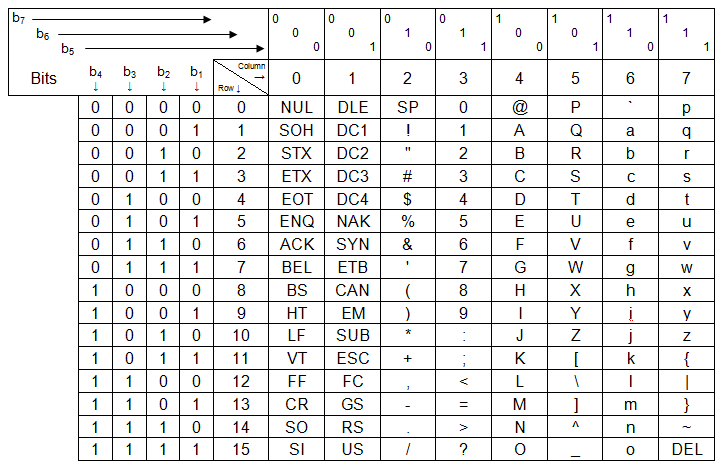
\includegraphics[scale=0.6]{./figures/ASCII.png}
  \caption{Encodage ASCII}
\end{figure}

\subsection{Code alphanumérique UTF-8}
Le code UTF-8 peut être vu comme une évolution majeure du code ASCII ; il vise à fournir un "répertoire universel de caractères codés", tout en conservant une retro-compatibilité avec
l'ASCII. Les symboles représentables en UTF8 englobent par exemple des caractères issus de langues étrangères (grec, hébreux, hiraganas japonais, etc), voire des musicaux (clé de sol, etc). L'UTF8 est, en 2017, utilisé par près de 90\% des sites web. Techniquement, un code UTF8 se présente comme une suite de 1 à 4 octets. Le nombre précis d'octets constitutifs
d'un code est lui-même encodé dans les bits de poids fort du code. Par exemple, lorsque le MSB vaut '0', cela signifie qu'un seul octet est nécessaire : cela correspond au code ASCII (il reste donc
7 bits pour coder les 128 caractères représentables en ASCII). Pour les codes au delà de l'ASCII, c'est le nombre de '1' en tête ("leading ones") du premier octet qui indique le nombre
d'octets qui suivront : par exemple un code UTF8 qui commence par "11110xxx" indique que le symbole codé nécessite 4 octets. Chaque octet suivant commence par "10".

\begin{center}
  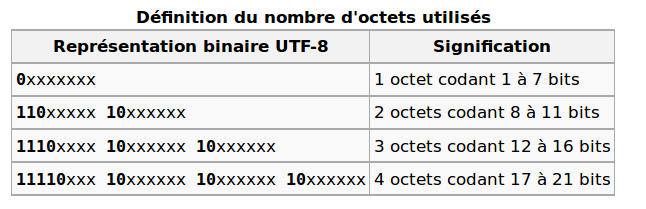
\includegraphics[scale=0.5]{./figures/utf8-w.png}
\end{center}

\begin{center}
  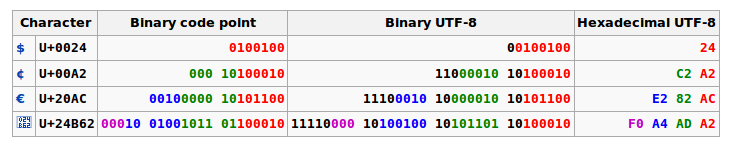
\includegraphics[scale=0.5]{./figures/utf8-example.png}
\end{center}
%===========================================================================================================
\section{Calcul en virgule fixe et en virgule flottante}

\subsection{Les nombres en virgule fixe}
Nous avons déja vu que les nombres qui possèdent une partie fractionnaire c'est-à-dire qui présentent une virgule après la partie
entière peuvent également se représenter en binaire ou dans tout autre base. On utilise simplement les puissances négatives de la
base en question.

$$ x = \sum_{i=-\infty}^{i=\infty} c_i.r^i, \mbox{avec } c_i \in \{0\dots (r-1)\} $$

En binaire, ces extensions s'appellent les ``décimales binaires'' : la première décimale binaire est $\frac{1}{2}$,
la seconde est $\frac{1}{4}$, la troisième est $\frac{1}{8}$ et ainsi de suite.\\

Dans certains processeurs de traitement du signal, on utilise une représentation des nombres dite {\it en virgule fixe} :
on restreint cette extension à une puissance donnée, afin que les opérations se fassent avec une position établie de la virgule
fixée, une bonne fois pour toute, ce qui simplifie l'architecture physique de l'unité de calcul. La position de la virgule est
alors connue et admise, au point où on peut l'oublier : cela revient à manipuler un simple entier. Par exemple, on peut associer
le nombre 125 à une mesure de 1.250 m. Pour une virgule placée au rang $k$, la différence entre deux nombres consécutifs
(appelée résolution) est égale $2^{-k}$ et sa dynamique (différence entre le nombre le plus grand et le plus petit) est réduite
à $2^{n-k}$, $n$ étant le nombre de bits du nombre.\\

Le calcul en virgule fixe est idéal dans le cas de l'addition : la place de la virgule n'est pas appelée à changer dans le
résultat. Ce n'est pas le cas de la mulitplication : pour deux nombres ayant 1 chiffre après la virgule, on obtient un résultat
qui possède 2 chiffres après la virgule. Il en est de même de 2 nombres de 2 chiffres chacun : le résultat est sur 4 chiffres,
ce qui peut provoquer des débordements. Enfin, deux nombres de 2 digits présentant une virgule à l'extrême gauche donneront un
résultat de multiplication à 4 chiffres après la virgule : il faudra tronquer le résultat...Bref : il est peut-être souhaitable
de conserver une liberté dans la gestion des virgules, quand cela est possible.

\subsection{Les nombres en virgule flottante. Norme IEEE 754}
Le calcul scientifique nous amène à des formules qui mélangent différents ordres de grandeur, peu compatibles avec
la représentation en virgule fixe. Les ordinateurs possèdent pour la plupart une unité en virgule flottante ; c'est
désormais le cas de 100\% des ordinateurs de bureau. Seuls certains processeurs embarqués n'en possèdent pas, car
l'unité de calcul flottante est consommatrice de surface. La représentation en virgule flottante est normalisée par
l'organisme IEEE, responsable de la standardisation de bon nombre de techniques, langages etc. Il s'agit ici de
s'assurer que les manipulations flottantes d'un programme ne dépendront pas de l'architecture de la machine : Intel,
AMD et. doivent fournir la même représentation. Il existe en réalité deux représentations normalisées IEEE 854 :
simple et double précision. On ne s'attarde ici que sur la première représentation.\\

\begin{center}
 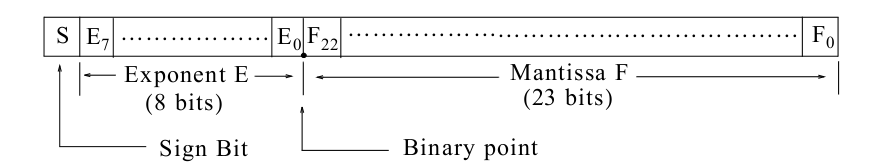
\includegraphics[scale=0.3]{./figures/ieee_854.png}
\end{center}

La représentation des flottants selon la norme IEEE simple précision se fait à l'aide de mots de 32 bits, ainsi constitués :
\begin{itemize}
\item un bit de signe, dénoté S : le $0$ représente le $+$ et le $1$ le $-$.
\item 8 bits d'exposant (7 à 0), dénoté $e$
\item 23 bits pour la partie fractionnaire, ou \textbf{mantisse} $f$, dénotés de 22 à 0. {\it e} et {\it f} sont toujours représentés en base 2, \underline{non complémentés à 2}.
\end{itemize}

La valeur absolue du nombre à représenter est normalisée selon la forme $1.f\times 2^e$. On notera que le premier '1' apparaissant dans cette forme n'est pas stocké, mais implicite.
Les 8 bits d'exposant présentent quelques particularités :
\begin{itemize}
  \item Les valeurs $00_{16}...FF_{16}$ représentent des codes spéciaux.
  \item Les valeurs $01_{16}...FE_{16}$ représentent des exposants courant de $2^{-126}$ à $2^{127}$.
  \item La valeur pôle est $7F_{16}=2^0=1$
\end{itemize}

\paragraph{Exemple}
Calculons la représentation du nombre $-3.25$ en IEEE 754-SP. On a : $-3.25=-11.01_2=-1.101 \times 2^1$
\begin{itemize}
  \item $s=1$
  \item $e=1+127=128=10000000_2$
  \item $f=10100000000000000000000$
\end{itemize}
D'où : $-3.25=11000000010100000000000000000000=c0500000_{16}$

\section{Manipulations numériques}

L'essentiel des techniques en logiciel embarqué consiste en des manipulations de {\it champs de bits} (bitfields), insérés au sein des nombres.
Un périphérique, par exemple, peut présenter au processeur plusieurs données dans un seul mot de 32 bits.

\subsection{Récupération d'un champ : masque hexadécimal}
Revenons à la représentation de la position (x,y).
Bien entendu, lorsque l'on utilise le nombre particulier Pos précédent,
il est nécessaire de connaître le mécanisme qui l'a créé, afin de récupérer
une coordonnée x ou y :
\begin{lstlisting}[
    label=listing:RubyTest,frame=single,
    float=h,
    caption=utilisation d'un masque hexadécimal en C,
    firstnumber=1,
    language=Ruby,
    basicstyle=\ttfamily,
    keywordstyle=\color{red},
    stringstyle=\color{blue}]
y = (0x0000FF) && Coord
\end{lstlisting}

Ce calcul permet d'extraire y du nombre Coord.
C'est un ET binaire, bit à bit, entre Coord et une constante exprimée en headecimal.
$0x0000FF$ a été créé de manière à annuler la contribution des bits de x dans Coord.
Pour cela les 4 digits hexadéciamaux sont effectivement à 0 ; ils représentent 16 bits
(4 fois 4 quartets) à 0. Quel que soit la valeur x, le ET bit à bit retournera des bits
à 0. A l'inverse, les 2 derniers quartets de la constante sont à $F$ et représentent
 donc 8 bits à 1. En conséquence, sur les 2 derniers quartets résultats, on retrouvera
 bien forcément la valeur de y, et elle seule, dans le résultat.



\subsection{Autres manipulations logicielles, au niveau bit}
La section précédente nous a permis de récupérer un champ particulier d'une donnée composée, grâce à une
 manipulation de bits. Il existe en fait de nombreuses manipulations qu'il est utile de connaître, notamment
 dans le domaine de la programmation pour des systèmes embarqués : les processeurs (et en particulier les micro-contrôleurs)
 actionnent et agissent sur leur environnement en écrivant et lisant des données précises stockées dans des circuits spéciaux appelés
 {\it registres}.

 A titre d'exemple, on propose un code écrit en langage C \footnote{Le langage C sera étudié en seconde année, pour les options STIC}
 qui réalise une boucle typique d'un système embarqué : la lecture d'une valeur détenue par un capteur (ici de simples boutons !),
suivie d'une action sur l'environnement, à savoir ici l'écriture des états des boutons sur des LEDs.

\begin{lstlisting}[language=C,frame=single]
#define Pushbuttons ((volatile long *) 0x10000050)
#define LEDS ((volatile long *) 0x10000010)
int main(void){
  long PBVal;
  while(1){
    PBVal = * Pushbuttons; // get the status of buttons : high or low
    *LEDS = PBVal; // display the status on LEDs
  }
}
\end{lstlisting}

 Pour les plus curieux  et à titre d'exemple, on donne ici une fonction (toujours écrite en langage C), qui permet d'initialiser (à 0) un registre particulier accessible par un micprocesseur.
 L'addresse du registre est ici $e0028008$. On indique au compilateur que ce registre n'est pas de son ressort à travers le mot clé "volatile" : le compilateur ne cherchera pas à réaliser
 d'optimisation sur ce registre. On accède au contenu par un {\it pointeur} (variable particulière qui contient l'addresse en question).

 \begin{lstlisting}[language=C,frame=single]
void clearReg(){
  (*((volatile unsigned int *) 0xe0028008))=0;
}
 \end{lstlisting}

 Ces registres sont à l'image de l'exemple de la position $(x,y)$, agglomérant plusieurs informations
 : par exemple, une alarme peut se manifester dans un bit de ce registre, à une position donnée (ex : le bit 7 du
 registre ``alarmes'' peut signifier ``porte non-verrouillée''). Il est donc important d'accéder à chacun des bits ou
 champs entiers de ces registres.

Le listing suivant propose quelques manipulations de champs de bits (applicables à à peu près tous les langages de programmations classiques).

\begin{lstlisting}[
    label=listing:RubyTest,frame=single,
    float=h,
    caption=Accès aux bits par programme informatique,
    firstnumber=1,
    language=C,
    basicstyle=\ttfamily,
    keywordstyle=\color{red},
    stringstyle=\color{blue}]
a = a | 0x4; /* mise a 1 du bit 2 de la variable a*/
a |=0x4; /* idem*/
b &= ~(0x4) /* mise a 0 du bit 2 */
b &= ~(1 << 2) /* idem, mais plus explicite*/
c ^= ~(1 << 5) /* inversion du bit 5*/
e >>=2 /* division de e par 4 */
\end{lstlisting}
% clear
% toggle
% divide



\subsection{Conversions et programmation}
Nous avons établi que $C_{2,3}(-2_{10})=6_{10}=110_2$. Comment trouver ces représentations,
à l'aide d'un langage de programmation s'exécutant sur votre ordinateur ? On peut écrire :

\begin{lstlisting}[
    label=listing:RubyTest,frame=single,
    float=h,
    caption=conversion signé vers non signé sur un nombre de bits restreint en langage Ruby,
    firstnumber=1,
    language=Ruby,
    basicstyle=\ttfamily,
    keywordstyle=\color{red},
    stringstyle=\color{blue}]
x = -2            % valeur a convertir
u = -2 & (2**3-1) % obtention de la valeur non signee. u=6
s = u.to_s(2)     % conversion en chaine de caracteres. s="110"
\end{lstlisting}

Pour comprendre cette manipulation, il faut savoir que les entiers signés sont codés sur 32 bits. Par conséquent, on peut établir
que la valeur $-2$ est représentée commme : $11\dots110_2$.

La seconde ligne consiste à masquer tous les bits au delà du troisième bit. Ces bits sont à 1, car ils représentent le bit
de signe.

\section{Vers la détection d'erreur entre émetteur et récepteur : bit de parité}
Lors de la transmission d'une donnée binaire codée sur plusieurs bits, il est fréquent que l'on lui adjoigne un bit supplémentaire, appelé {\it bit de parité}.
La valeur $0$ ou $1$ dépend des autres bits, de manière à ce que la somme totale des $1$ du code binaire soit paire. Ceci permet, à moindre frais, de s'assurer qu'une
erreur (simple) ne s'est pas produite lors de la transmission. En effet, le recepteur peut alors verifier la parité de la donnée reçue. L'hypothèse sous-jacente stipule
qu'une seule erreur binaire est tolérée. Au delà, il faudra rajouter des bits plus sophistiqués : code de Hamming, Turbo-codes etc.

\begin{figure}[htb!]
    \centering
    \begin{minipage}{0.45\textwidth}
        \centering
        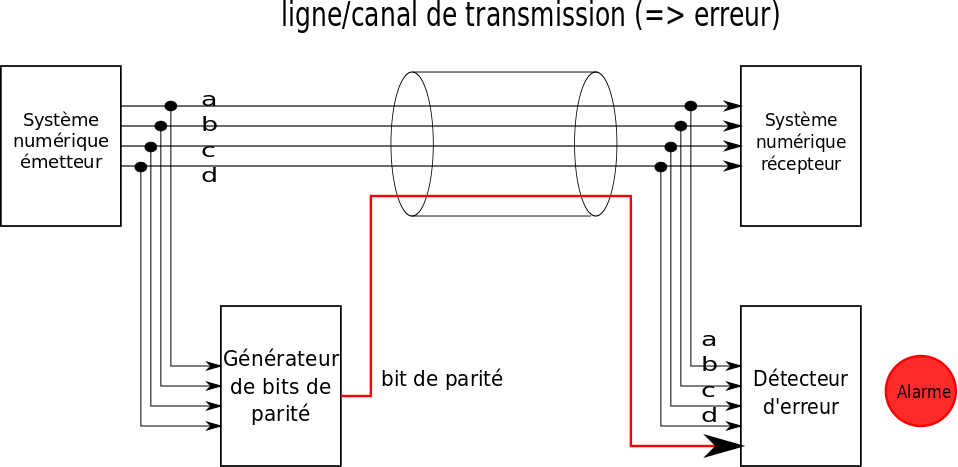
\includegraphics[width=1.1\textwidth]{./figures/parite-1.png} % first figure itself
        \caption{Emetteur, récepteur et canal bruité}
    \end{minipage}\hfill
    \begin{minipage}{0.45\textwidth}
        \centering
        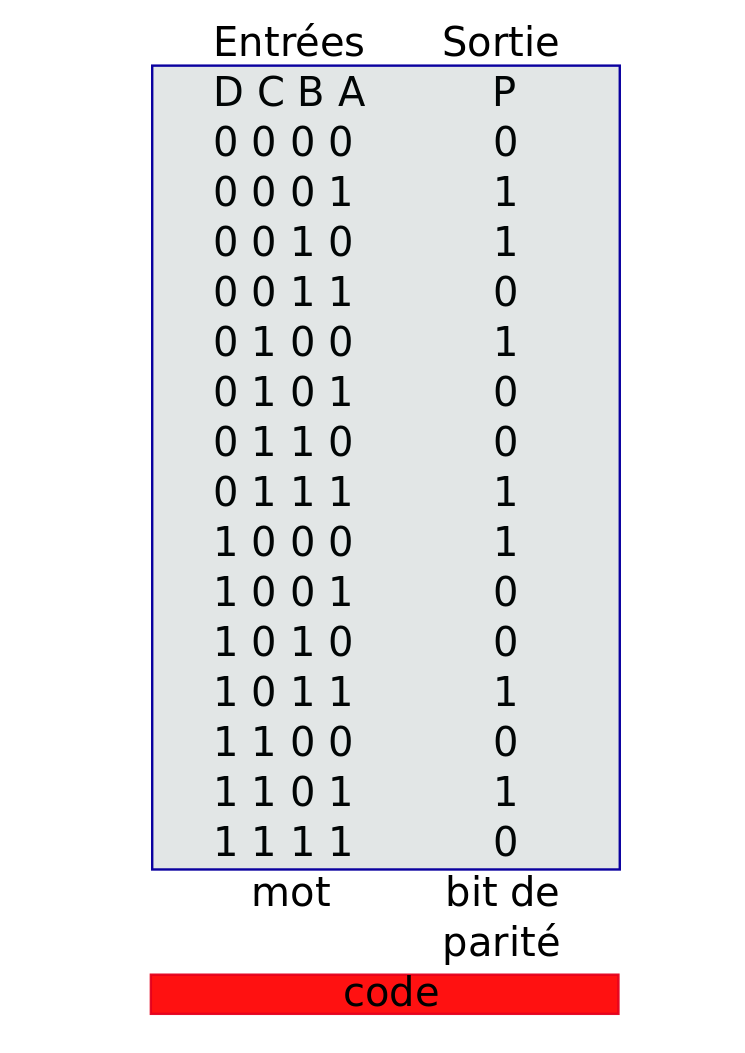
\includegraphics[width=0.4\textwidth]{./figures/parite-3.png} % second figure itself
        \caption{Table de vérité du bit de parité}
    \end{minipage}
\end{figure}


\section{Conclusion}
Ce chapitre vous a permi de rentrer de plain-pied dans les représentations numériques,
notamment avec la prise de connaissance de différents codes. Ce domaine est vaste ! Il existe d'autres codes
que nous n'avons pas aborder, comme les codes en excès de 3 où le code de Aïken.
Nous nous appuyerons sur ces premières connaissances afin de construire --bientôt-- nos
premières applications numériques.
Nous recommandons ici, en complément, la lecture de Bryant et O'Hallaron \cite{Bryant:2010:CSP:1841497} pour plus de détails sur la partie arithmétique.
Il est également intéressant de regarder d'autres présentations orientées sur la Théorie de l'Information comme Cover \& Thomas \cite{Cover:2006:EIT:1146355}.
